\documentclass[letterpaper,12pt,fleqn]{article}
\usepackage{matharticle}
\usepackage{tikz}
\usepackage{graphicx}
\usepackage{siunitx}
\pagestyle{empty}
\newcommand{\e}{\varepsilon}
\begin{document}

\section*{Arbitrarily Close}

The difference between algebra and calculus is a concept called \emph{arbitrarily close}.  You have already seen this
concept at work with things like asymptotes and the infinite repeating decimal form of some rational numbers
(e.g., \(0.11111\ldots=\frac{1}{9}\)).  To develop this concept more formally, we need to establish the concepts of
\emph{distance} and \emph{arbitrarily small} first.

\subsection*{Distance}

Consider two points on the number line, say \(2\) and \(5\):

\bigskip

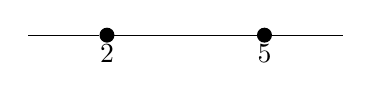
\begin{tikzpicture}
  \node (a) [draw,circle,fill,inner sep=0pt,minimum size=5pt] at (1,0) {};
  \node (b) [draw,circle,fill,inner sep=0pt,minimum size=5pt] at (3,0) {};
  \draw (0,0) to (a) to (b) to (4,0);
  \node [below] at (a) {2};
  \node [below] at (b) {5};
\end{tikzpicture}

\bigskip

To find the distance between two points, we subtract the destination from the source:
\[d(2,5)=5-2=3\]
How about the distance from \(5\) to \(2\)?:
\[d(5,2)=2-5=-3\]
But distance should be non-negative and should be the same, no matter which direction you go (note that this is
different from \emph{displacement}, which is signed).  So how do we ignore the negative sign?

Recall from Section 0.1, Real Numbers: Order and Absolute Value, p7:

\begin{definition}[Distance]
  Let \(a,b\in\R\) be two real numbers on the real number line.  The \emph{distance} between \(a\) and \(b\), which
  is the same as the distance between \(b\) and \(a\), is given by:
  \[\abs{b-a}=\abs{a-b}\]
\end{definition}

In fact, this is the only time when subtraction is commutative: when it is in an absolute value.

\subsection*{Arbitrarily Small}

We have already dealt with the concept of \(\infty\) as an \emph{arbitrarily large} value.  Instead, we introduce
\(\e\), the Greek letter epsilon, to refer to an \emph{arbitrarily small} value.  This means that \(\e\) is not
some particular value, instead it refers to a process of getting progressively smaller but not quite \(0\), just
like infinity refers to the process of getting progressively larger.

For example, if I ask you for a small value and you say \(0.1\).  But I say, no smaller, so you say \(0.001\), but
I want it smaller still so you say \(0.0000001\), but again, I say smaller, and so on in an infinite pattern.  Note
that the number of steps is arbitrarily large; however, the values of \(\e\) get arbitrarily small.

But how do I know that I can alway pick a smaller value greater than \(0\)?  Consider a subset of the number line
from \(0\) to \(1\):

\bigskip

\begin{tikzpicture}
  \draw (0,0) to (3,0);
  \draw (0,0.1) to (0,-0.1);
  \draw (3,0.1) to (3,-0.1);
  \node at (0,0) [below] {\(0\)};
  \node at (3,0) [below] {\(1\)};
\end{tikzpicture}

\bigskip

How many real values are there between \(0\) and \(1\)?  An infinite number!  In fact, between any two real numbers
there exists and infinite number of real numbers, so we can always pick one: 0.5, 0.1, 0.01, 0.000001, etc.

\bigskip

\begin{tikzpicture}
  \draw (0,0) to (3,0);
  \draw (0,0.1) to (0,-0.1);
  \draw (1.5,0.1) to (1.5,-0.1);
  \draw (0.3,0.1) to (0.3,-0.1);
  \draw (0.1,0.1) to (0.1,-0.1);
  \draw (3,0.1) to (3,-0.1);
  \node at (0,0) [below] {\(0\)};
  \node at (3,0) [below] {\(1\)};
\end{tikzpicture}

\subsection*{Arbitrarily Small Interval}

Now, suppose we have a fixed point \(a\), say 2, and some arbitrarily small \(\e\).  We use these values to
construct the following interval: \([2-\e,2+\e]\), where each endpoint is distance \(\e\) from the base value of
\(2\):

\bigskip

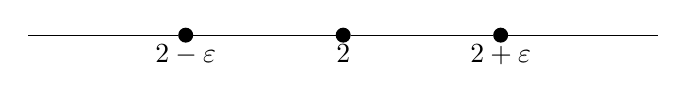
\begin{tikzpicture}
  \node (a) [draw,circle,fill,inner sep=0pt,minimum size=5pt] at (0,0) {};
  \node (b) [draw,circle,fill,inner sep=0pt,minimum size=5pt] at (-2,0) {};
  \node (c) [draw,circle,fill,inner sep=0pt,minimum size=5pt] at (2,0) {};
  \draw (-4,0) to (b) to (a) to (c) to (4,0);
  \node [below] at (a) {\(2\)};
  \node [below] at (b) {\(2-\e\)};
  \node [below] at (c) {\(2+\e\)};
\end{tikzpicture}

We now want to locate other values \(x\) in relation to our base value and our interval.  There are three
possibilities:

\begin{enumerate}
\item \(x\) \emph{coincides} with one of the endpoints and thus is exactly \(\e\) away from the base point:
  \(\abs{x-a}=\e\).

  \begin{minipage}{3in}
    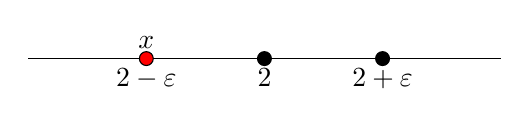
\begin{tikzpicture}[scale=0.75]
      \node (a) [draw,circle,fill,inner sep=0pt,minimum size=5pt] at (0,0) {};
      \node (b) [draw,circle,fill=red,inner sep=0pt,minimum size=5pt] at (-2,0) {};
      \node (c) [draw,circle,fill,inner sep=0pt,minimum size=5pt] at (2,0) {};
      \draw (-4,0) to (b) to (a) to (c) to (4,0);
      \node [below] at (a) {\(2\)};
      \node [below] at (b) {\(2-\e\)};
      \node [above] at (b) {\(x\)};
      \node [below] at (c) {\(2+\e\)};
    \end{tikzpicture}
  \end{minipage}
  \begin{minipage}{3in}
    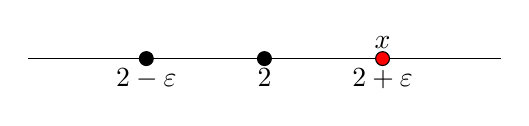
\begin{tikzpicture}[scale=0.75]
      \node (a) [draw,circle,fill,inner sep=0pt,minimum size=5pt] at (0,0) {};
      \node (b) [draw,circle,fill,inner sep=0pt,minimum size=5pt] at (-2,0) {};
      \node (c) [draw,circle,fill=red,inner sep=0pt,minimum size=5pt] at (2,0) {};
      \draw (-4,0) to (b) to (a) to (c) to (4,0);
      \node [below] at (a) {\(2\)};
      \node [below] at (b) {\(2-\e\)};
      \node [below] at (c) {\(2+\e\)};
      \node [above] at (c) {\(x\)};
    \end{tikzpicture}
  \end{minipage}

  This corresponds to absolute value linear equations as presented in Section 1.5.
  
\item \(x\) is \emph{outside} the interval and thus is greater than \(\e\) away from the base point:
  \(\abs{x-a}>\e\).

  \begin{minipage}{3in}
    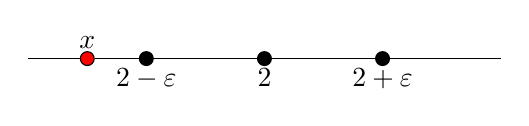
\begin{tikzpicture}[scale=0.75]
      \node (a) [draw,circle,fill,inner sep=0pt,minimum size=5pt] at (0,0) {};
      \node (x) [draw,circle,fill=red,inner sep=0pt,minimum size=5pt] at (-3,0) {};
      \node (b) [draw,circle,fill,inner sep=0pt,minimum size=5pt] at (-2,0) {};
      \node (c) [draw,circle,fill,inner sep=0pt,minimum size=5pt] at (2,0) {};
      \draw (-4,0) to (x) to (b) to (a) to (c) to (4,0);
      \node [below] at (a) {\(2\)};
      \node [above] at (x) {\(x\)};
      \node [below] at (b) {\(2-\e\)};
      \node [below] at (c) {\(2+\e\)};
    \end{tikzpicture}
  \end{minipage}
  \begin{minipage}{3in}
    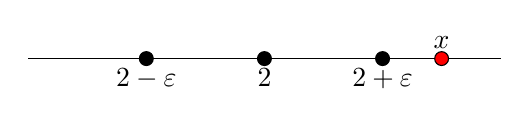
\begin{tikzpicture}[scale=0.75]
      \node (a) [draw,circle,fill,inner sep=0pt,minimum size=5pt] at (0,0) {};
      \node (b) [draw,circle,fill,inner sep=0pt,minimum size=5pt] at (-2,0) {};
      \node (c) [draw,circle,fill,inner sep=0pt,minimum size=5pt] at (2,0) {};
      \node (x) [draw,circle,fill=red,inner sep=0pt,minimum size=5pt] at (3,0) {};
      \draw (-4,0) to (b) to (a) to (c) to (x) to (4,0);
      \node [below] at (a) {\(2\)};
      \node [below] at (b) {\(2-\e\)};
      \node [below] at (c) {\(2+\e\)};
      \node [above] at (x) {\(x\)};
    \end{tikzpicture}
  \end{minipage}

  This corresponds to absolute value linear inequalities as presented in Section 1.6.
  
\item \(x\) is \emph{inside} the interval and thus is less than \(\e\) away from the base point: \(\abs{x-a}>\e\).

  \begin{minipage}{3in}
    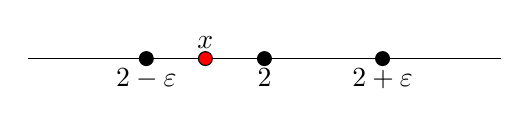
\begin{tikzpicture}[scale=0.75]
      \node (a) [draw,circle,fill,inner sep=0pt,minimum size=5pt] at (0,0) {};
      \node (b) [draw,circle,fill,inner sep=0pt,minimum size=5pt] at (-2,0) {};
      \node (x) [draw,circle,fill=red,inner sep=0pt,minimum size=5pt] at (-1,0) {};
      \node (c) [draw,circle,fill,inner sep=0pt,minimum size=5pt] at (2,0) {};
      \draw (-4,0) to (b) to (x) to (a) to (c) to (4,0);
      \node [below] at (a) {\(2\)};
      \node [below] at (b) {\(2-\e\)};
      \node [above] at (x) {\(x\)};
      \node [below] at (c) {\(2+\e\)};
    \end{tikzpicture}
  \end{minipage}
  \begin{minipage}{3in}
    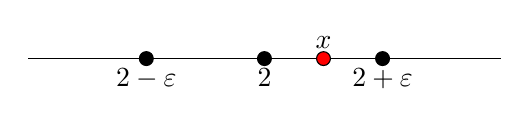
\begin{tikzpicture}[scale=0.75]
      \node (a) [draw,circle,fill,inner sep=0pt,minimum size=5pt] at (0,0) {};
      \node (b) [draw,circle,fill,inner sep=0pt,minimum size=5pt] at (-2,0) {};
      \node (x) [draw,circle,fill=red,inner sep=0pt,minimum size=5pt] at (1,0) {};
      \node (c) [draw,circle,fill,inner sep=0pt,minimum size=5pt] at (2,0) {};
      \draw (-4,0) to (b) to (a) to (x) to (c) to (4,0);
      \node [below] at (a) {\(2\)};
      \node [below] at (b) {\(2-\e\)};
      \node [above] at (x) {\(x\)};
      \node [below] at (c) {\(2+\e\)};
    \end{tikzpicture}
  \end{minipage}

  This also corresponds to absolute value linear inequalities as presented in Section 1.6, and it is in fact the
  case that we are interested in for our definition of \emph{arbitrarily close}.
\end{enumerate}

\subsection*{Arbitrarily Close}

Consider the interval represented by the absolute value inequality:
\[\abs{x-a}<\e\]
As \(\e\) gets arbitrarily small, denoted by: \(\e\to0\), the values of \(x\) that we can choose inside the
interval get closer and closer to the base value \(a\).  Since \(\e>0\) we are never forced onto \(a\), just
\emph{arbitrarily close} to it!

\begin{example}
  \begin{enumerate}[left=0pt]
  \item []
  \item Let our base point \(a=2\) and start with \(\e=0.1\).  Pick \(x=2.05\):

    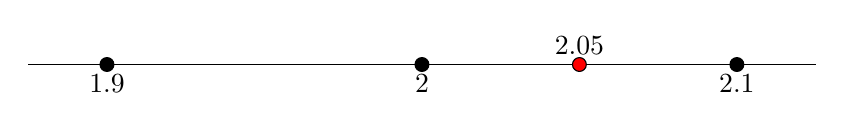
\begin{tikzpicture}
      \draw (0,0) -- (10,0);
      \node (a) [draw,circle,fill,inner sep=0pt,minimum size=5pt] at (5,0) {};
      \node (b) [draw,circle,fill,inner sep=0pt,minimum size=5pt] at (1,0) {};
      \node (x) [draw,circle,fill=red,inner sep=0pt,minimum size=5pt] at (7,0) {};
      \node (c) [draw,circle,fill,inner sep=0pt,minimum size=5pt] at (9,0) {};
      \node [below] at (a) {\(2\)};
      \node [below] at (b) {\(1.9\)};
      \node [above] at (x) {\(2.05\)};
      \node [below] at (c) {\(2.1\)};
    \end{tikzpicture}
    \[\abs{2.05-2}=0.05<0.1=\e\]

  \item Now, let \(\e=0.04\) and pick \(x=2.01\):

    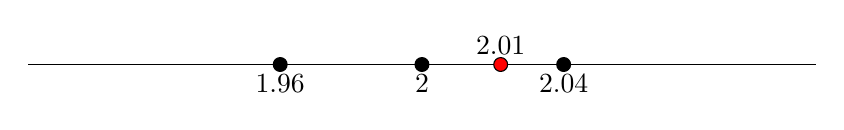
\begin{tikzpicture}
      \draw (0,0) -- (10,0);
      \node (a) [draw,circle,fill,inner sep=0pt,minimum size=5pt] at (5,0) {};
      \node (b) [draw,circle,fill,inner sep=0pt,minimum size=5pt] at (3.2,0) {};
      \node (x) [draw,circle,fill=red,inner sep=0pt,minimum size=5pt] at (6,0) {};
      \node (c) [draw,circle,fill,inner sep=0pt,minimum size=5pt] at (6.8,0) {};
      \node [below] at (a) {\(2\)};
      \node [below] at (b) {\(1.96\)};
      \node [above] at (x) {\(2.01\)};
      \node [below] at (c) {\(2.04\)};
    \end{tikzpicture}
    \[\abs{2.01-2}=0.01<0.04=\e\]

  \item Note that \(x\) need not always be on the same side.  This time, let \(\e=0.03\) and pick \(x=1.99\):

    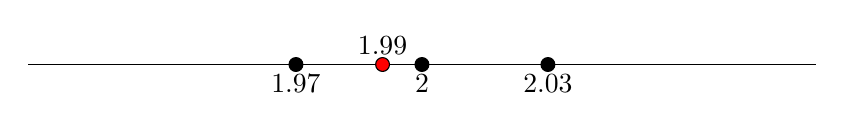
\begin{tikzpicture}
      \draw (0,0) -- (10,0);
      \node (a) [draw,circle,fill,inner sep=0pt,minimum size=5pt] at (5,0) {};
      \node (b) [draw,circle,fill,inner sep=0pt,minimum size=5pt] at (3.4,0) {};
      \node (x) [draw,circle,fill=red,inner sep=0pt,minimum size=5pt] at (4.5,0) {};
      \node (c) [draw,circle,fill,inner sep=0pt,minimum size=5pt] at (6.6,0) {};
      \node [below] at (a) {\(2\)};
      \node [below] at (b) {\(1.97\)};
      \node [above] at (x) {\(1.99\)};
      \node [below] at (c) {\(2.03\)};
    \end{tikzpicture}
    \[\abs{1.99-2}=0.01<0.03=\e\]

  \item Nor does each step have to get closer: it just needs to be within the new smaller interval.  This time, let
    \(e=0.02\) and pick \(x=1.985\):

    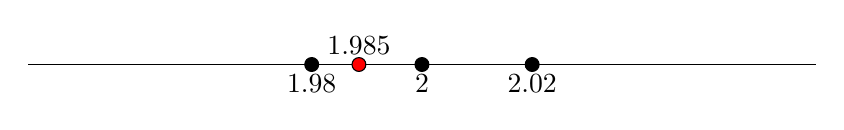
\begin{tikzpicture}
      \draw (0,0) -- (10,0);
      \node (a) [draw,circle,fill,inner sep=0pt,minimum size=5pt] at (5,0) {};
      \node (b) [draw,circle,fill,inner sep=0pt,minimum size=5pt] at (3.6,0) {};
      \node (x) [draw,circle,fill=red,inner sep=0pt,minimum size=5pt] at (4.2,0) {};
      \node (c) [draw,circle,fill,inner sep=0pt,minimum size=5pt] at (6.4,0) {};
      \node [below] at (a) {\(2\)};
      \node [below] at (b) {\(1.98\)};
      \node [above] at (x) {\(1.985\)};
      \node [below] at (c) {\(2.02\)};
    \end{tikzpicture}
    \[\abs{1.985-2}=0.015<0.02=\e\]

  \item But eventually, we are forced to pick smaller values.  This time, let \(e=0.01\) and select \(x=2.005\):

    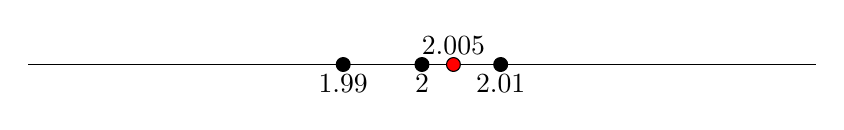
\begin{tikzpicture}
      \draw (0,0) -- (10,0);
      \node (a) [draw,circle,fill,inner sep=0pt,minimum size=5pt] at (5,0) {};
      \node (b) [draw,circle,fill,inner sep=0pt,minimum size=5pt] at (4.0,0) {};
      \node (x) [draw,circle,fill=red,inner sep=0pt,minimum size=5pt] at (5.4,0) {};
      \node (c) [draw,circle,fill,inner sep=0pt,minimum size=5pt] at (6.0,0) {};
      \node [below] at (a) {\(2\)};
      \node [below] at (b) {\(1.99\)};
      \node [above] at (x) {\(2.005\)};
      \node [below] at (c) {\(2.01\)};
    \end{tikzpicture}
    \[\abs{2.005-2}=0.005<0.01=\e\]
  \end{enumerate}
\end{example}

Thus, the \(x\) values that can be selected get \emph{arbitrarily close} to the base value \(a\) as \(\e\) gets
\emph{arbitrarily small}.  This can be stated in any of the following ways:
\begin{enumerate}
\item \(x\) gets arbitrarily close to \(a\) as \(e\) gets arbitrarily small
\item \(x\) \emph{converges} to \(a\) as \(e\to0\)
\item \(\abs{x-a}<\e\)
\item \(x\to a\) as \(e\to0\)
\end{enumerate}

\end{document}
